\documentclass[12pt]{article}
\usepackage{amsmath}
\usepackage{grffile}
\usepackage{graphicx}
\usepackage{pdfpages}
\usepackage{appendix}

\renewcommand*{\thesection}{\alph{section}.}

\author{Sundaresan G}
%\title{Advertisement No. CDS/KA/SERB-SRG/DEC2020/RA}
\begin{document}
	
\begin{titlepage}
	\begin{center}
		\vspace*{1cm}
		
		\textbf{\Large{Solution to the 1D Heat Equation}}
		
		\vspace{0.5cm}
		Advertisement No. CDS/KA/SERB-SRG/DEC2020/RA
		
		\vspace{1.5cm}
		
		A report submitted for the application of\\
		Project Assistant Position
		
		
		\vfill
		
		\textbf{\large{Sundaresan G}}\\
		Scientist/Engineer\\
		ISRO Propulsion Complex
		
		\vspace{0.8cm}
		
		B.Tech Mechanical Engineering\\
		Batch of 2016, NITT\\
		
	\end{center}
\end{titlepage}
\tableofcontents

	\section{Analytical Solution}
	\begin{center}
		\begin{tabular}{l l}
			Given problem & $u_t=u_{xx}$\\		
			Domain & $x=[0,1]$\\
			Boundary condition & $u(0,t)=u(1,t),\
			u_x(0,t)=u_x(1,t)$\\
			Initial condition & $u(x,0)=sin(2\pi x)$
		\end{tabular}
	\end{center}
	The given problem is a well posed homogenous linear PDE and has a unique solution for the given boundary (Neumann) and initial conditions.\\
	The solution is derived as follows by variable separation:\\
	
	\begin{tabular}{r l}
		Let & $u(x,t)=X(x)*T(t)$ \\
		& $u_t=u_{xx} \implies XT_t=X_{xx}T$ \\
		& ${X_{xx}\over X} = {T_t \over T} = \alpha$
		
				
	\end{tabular} \\
	($\alpha$ is a\ constant since LHS is only a function of x and RHS is a function of t)\\
	
	\begin{tabular}{l l}
		Case 1: & $\alpha = 0$ \\
		$\implies$ & $X=ax+b, \ T=c$ \\
		$\implies$ & $u^{\alpha=0}=a_1 x + a_2$
	\end{tabular} \\
	
	\begin{tabular}{l l}
		Case 2: & $\alpha = \beta^2 > 0$ \\
		$\implies$ & $X=ae^{\beta x}+be^{-\beta x}, \ T=ce^{\beta^2 t^2}$ \\
		$\implies$ & $u^{\alpha>0}=(b_1e^{\beta x}+b_2e^{-\beta x})e^{\beta^2 t^2}$
	\end{tabular} \\

	where $b_1$ and $b_2$ are arbitrary constants depending on $\beta$ \\
	
	\begin{tabular}{l l}
		Case 3: & $\alpha = -\lambda^2 < 0$ \\
		$\implies$ & $X=acos({\lambda x})+bsin({\lambda x}), \ T=ce^{-\lambda^2 t^2}$ \\
		$\implies$ & $u^{\alpha<0}=(c_1cos({\lambda x})+c_2sin({\lambda x}))e^{-\lambda^2 t^2}$
	\end{tabular} \\
	
	where $c_1$ and $c_2$ are arbitrary constants depending on $\lambda$ \\
	
	Due to the homogenous and linear nature of the given PDE, the solution is given by \\ \\ 
	
	\begin{tabular}{r l l}
		$u(x,t)$ &=& $a_1 x + a_2 + \sum_{\beta \in S_1}^{}((b_1(\beta)e^{\beta x}+b_2(\beta)e^{-\beta x})e^{\beta^2 t^2})$\\
		&& + $\sum_{\lambda \in S_2}^{}((c_1(\lambda)cos({\lambda x})+c_2(\lambda)sin({\lambda x}))e^{-\lambda^2 t^2})$
	\end{tabular} \\ \\ 
	where $S_1$ and $S_2$ are countable subsets of non-zero Real numbers (since the summation should converge) \\ 
	
	Now the solution is finite even for $t \to \infty$ (by Physics of the heat equation with no external energy source). Hence $b_1$ and $b_2$ should be 0 for any value of $\beta$. \\
	
	$u(x,t) = a_1 x + a_2 + \sum_{\lambda \in S_2}^{}((c_1(\lambda)cos({\lambda x})+c_2(\lambda)sin({\lambda x}))e^{-\lambda^2 t^2})$ \\
	
	Applying boundary condition $u(0,t) = u(1,t)$, we get \\
	
	$a_2 + \sum_{\lambda \in S_2}^{}((c_1(\lambda))e^{-\lambda^2 t^2}) = a_1 + a_2 + \sum_{\lambda \in S_2}^{}((c_1(\lambda)cos({\lambda })+c_2(\lambda)sin({\lambda}))e^{-\lambda^2 t^2})$
	
	$\implies a_1 + \sum_{\lambda \in S_2}^{}([c_1(\lambda)(cos({\lambda })-1)+c_2(\lambda)sin({\lambda})]e^{-\lambda^2 t^2}) = 0$ \\ 
	
	Since the above equation is true for any value of t, 
	
	\begin{center}
		$a_1 = 0$ \hspace{30mm} and
	\end{center}	
	\begin{equation} \label{eq1}
	c_1(\lambda)(cos({\lambda })-1)+c_2(\lambda)sin({\lambda}) = 0 \hspace{20mm}  \text{for every $\lambda \in S_2$}
	\end{equation} 
	
	Applying boundary condition $u_x(0,t)=u_x(1,t)$, we get \\
	
	$\sum_{\lambda \in S_2}^{}(\lambda c_2(\lambda))e^{-\lambda^2 t^2})= \sum_{\lambda \in S_2}^{}((-\lambda c_1(\lambda)sin(\lambda)+\lambda c_2(\lambda)cos(\lambda))e^{-\lambda^2 t^2})$ \\
	
	We know $\lambda \neq 0$ and the above equation is true for every t. Hence 	
	\begin{equation} \label{eq2}
	c_1(\lambda)sin(\lambda) + c_2(\lambda)(1-cos(\lambda))=0 \hspace{20mm}  \text{for every $\lambda \in S_2$}
	\end{equation}
	
	Solving equations \ref{eq1} and \ref{eq2}, we get the following two equations
	\begin{equation}
	c_1=c_2=0
	\end{equation}
	 The above equation leads to a trivial solution and does not satisfy the given initial condition.
	 
	 \begin{equation}
	 sin(\lambda)=(1-cos(\lambda))=0
	 \end{equation}
	
	The above equation is satisfied if and only if,
	
	\begin{equation}
	\lambda = n \pi, \\ \text{where n $\in$ Z}
	\end{equation}
	
	Substituting the results in the solution u(x,t) and combining the arbitrary constants,
	
	\begin{equation}
	u(x,t)=({A_0\over 2} +\sum_{n=1}^{\infty} (A_n cos(n \pi x)+ B_n sin(n \pi x)))e^{(-\lambda^2 t^2)} 
	\end{equation}
	
	Now for t=0,
	
	\begin{equation}
	u(x,0)={A_0\over 2} +\sum_{n=1}^{\infty} (A_n cos(n \pi x)+ B_n sin(n \pi x)) 
	\end{equation}
	
	The above equation is clearly in the form of Fourier series and hence the arbitrary constants are given by the following equations,
	
	\begin{equation}
	A_n = 2 \int_{0}^{1} u(x,0)cos (n \pi x) dx, \hspace{10mm}\text{n=0,1,2,...}
	\end{equation}
	
	\begin{equation}
	B_n = 2 \int_{0}^{1} u(x,0)sin (n \pi x) dx, \hspace{10mm}\text{n=1,2,...}
	\end{equation}
	
	For the given initial condition $u(x,0)=sin(2 \pi x)$, we get
	
	\begin{equation}
	A_n = 0 \hspace{10mm}\text{n=0,1,2,...}
	\end{equation}	
	
	\begin{equation}
	B_n = 0 \hspace{10mm}\text{n $\neq$ 2}
	\end{equation}
		
	\begin{equation}
	B_2 = 1
	\end{equation}
	
	Thus the analytical solution is given by
	
	\begin{equation}
	u(x,t)= sin(2 \pi x) e^{(-4 \pi^2 t^2)}
	\end{equation}
	
	The above solution satisfies the PDE, initial and boundary conditions. Moreover due to well posed nature of the problem, the solution obtained is a unique one.
	
	\section{Numerical Scheme}
	
	\begin{center}
		$u_t=u_{xx}$
	\end{center}
	
	The following is the explicit Euler (time derivative) and second order central difference (space derivative) scheme
	
	\begin{center}
		\begin{equation}
		u^{t+1}_{i}= u^t_i + {\Delta t \over (\Delta x)^2} (u^t_{i+1}-2u^t_i+u^t_{i-1})
		\end{equation} 
	\end{center}

	The above equation can be used to obtain the value at next time step for every internal point. For the end points, the following equations are used due to periodic boundary conditions,
	
	\begin{equation}
	u^{t+1}_{0}= u^t_0 + {\Delta t \over (\Delta x)^2} (u^t_{1}-2u^t_0+u^t_{endpoint-1})
	\end{equation} 
	
	\begin{equation}
	u^{t+1}_{endpoint}= u^{t+1}_0
	\end{equation}
	
	Since $\Delta t = 0.00001$ , the maximum number of grid points allowed is 223 due to convergence and stability criteria, $\Delta t \leq {1\over2}(\Delta x)^2$

	\section{Numerical simulations}
	
	A code is written in C language and given in Appendix A. It uses command line arguments for input of Number of grid points and Time step at which solution is required. Please compile it using a suitable compiler (GCC) as follows	
	\begin{center}
		\begin{tabular}{l}
			\textbf{gcc code.c -o "output file name"} \\
			\textbf{"output file name".exe "Number of grid points" "Time step(s)"}
		\end{tabular}
	\end{center}
	
	For example,
	
	\begin{center}
		\begin{tabular}{l}
			\textbf{gcc code.c -o results} \\
			\textbf{results.exe 200 300 500 1000}
		\end{tabular}
	\end{center}

	The above example inputs 200 as the number of grid points and prints the numerical and analytical solutions at 300, 500 and 1000 time steps. 

	\textbf{Note:} The maximum number of grid points (default:128) the code accepts is 220 (for convergence) and the maximum time step (default: 0, 100, 500 and 1000) is 3000 and number of time step arguments (default:4) is 10.

	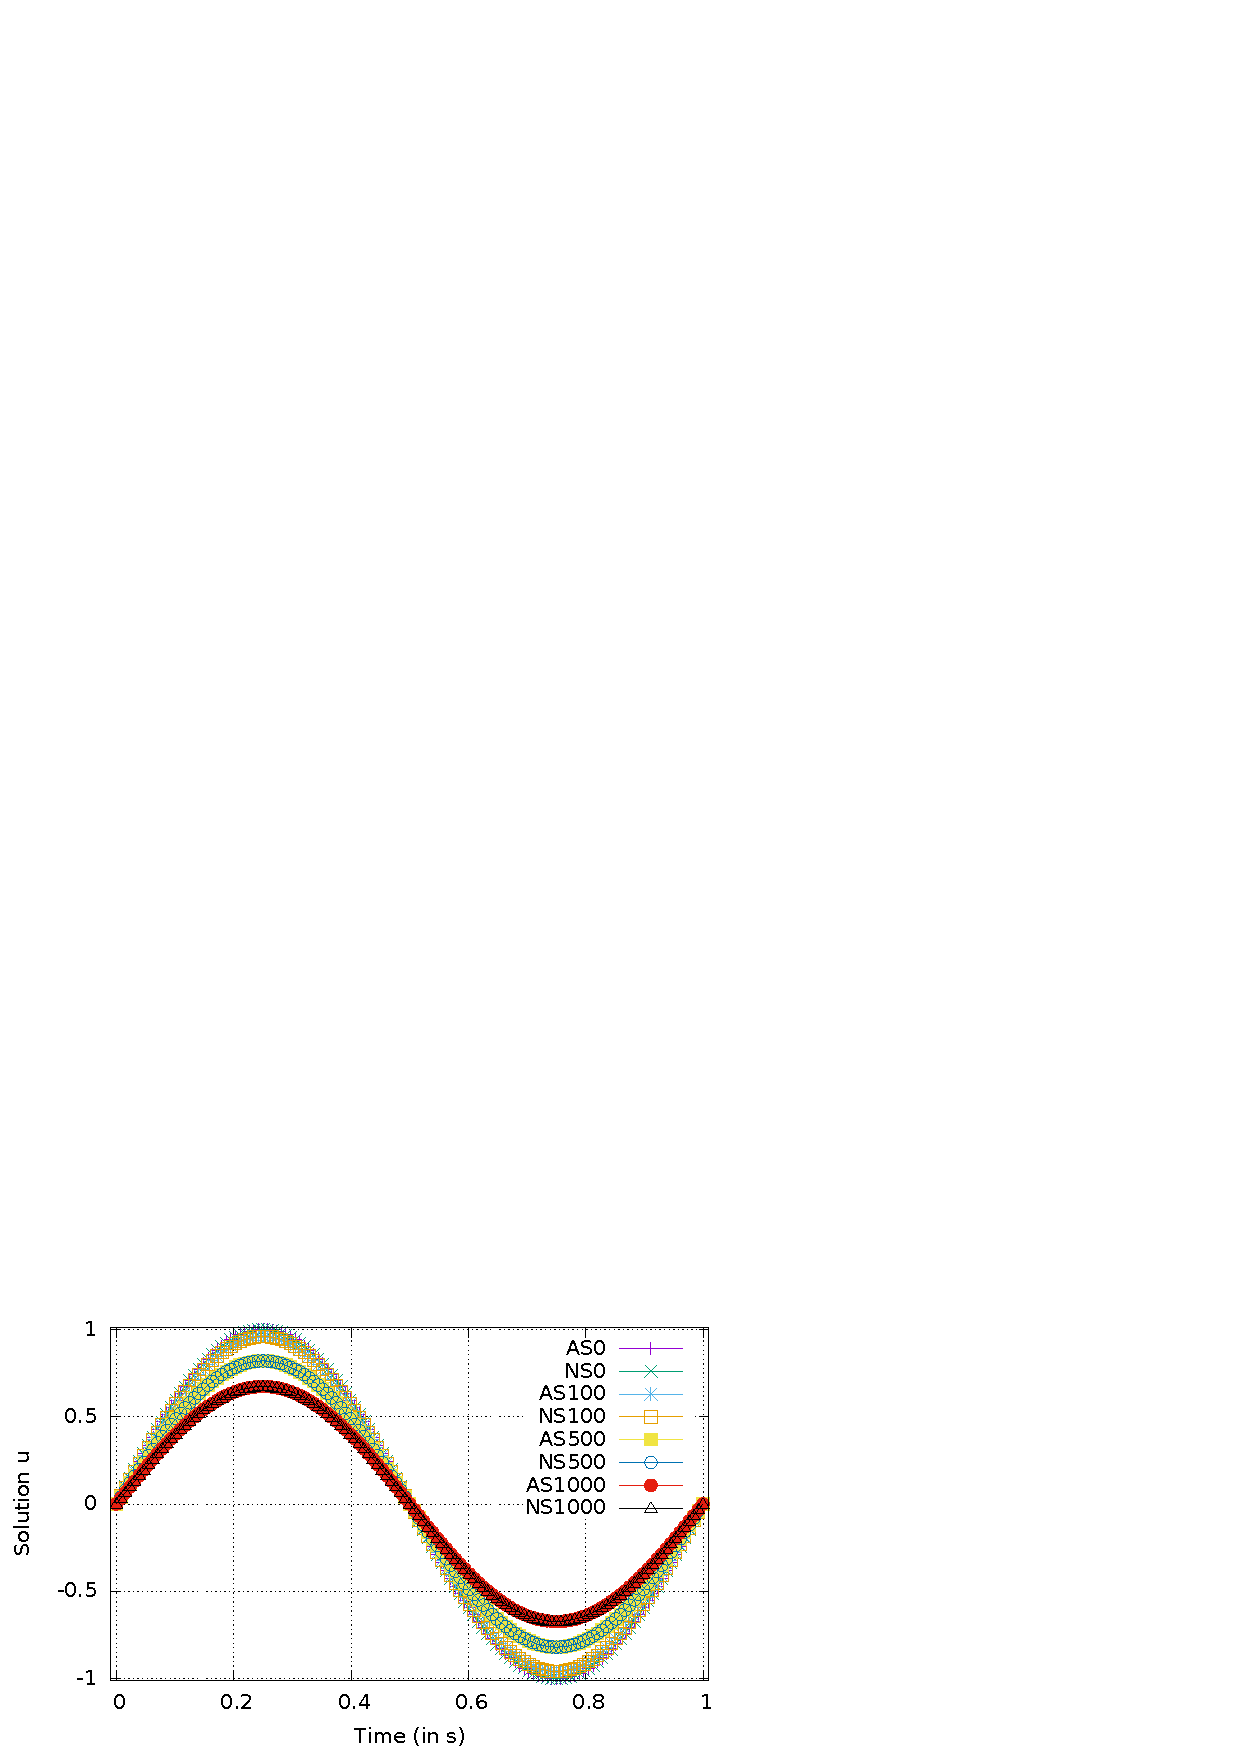
\includepdf[scale=0.65,pages=1, angle=90, pagecommand=\section{Solution Plot for 128 grid points}]{"D:/iisc project/1d-heat-eqn-solver-single-array/Gnuplot/NSvsAS_plot_for_128_grid_points.pdf"}
	
		%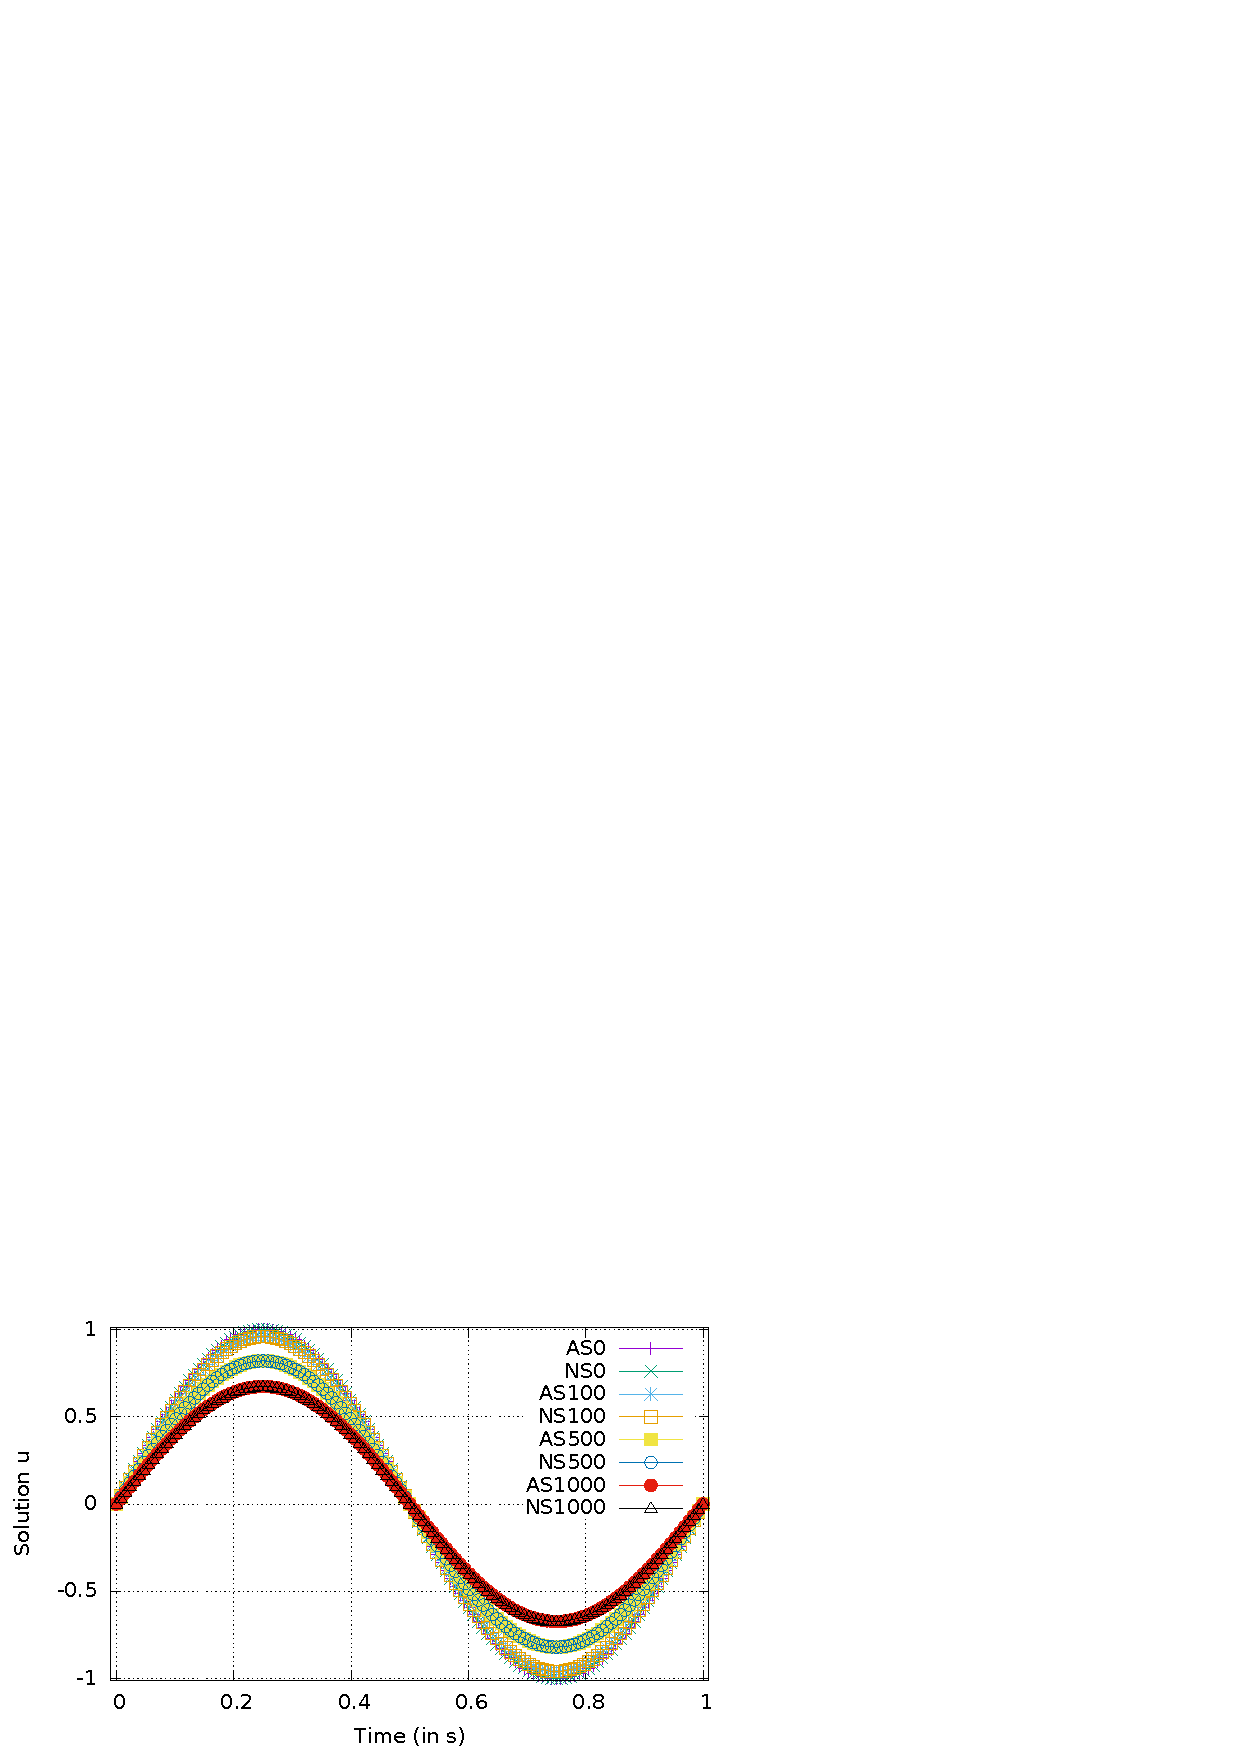
\includepdf[pages=-]{"D:/iisc project/1d-heat-eqn-solver-single-array/Gnuplot/NSvsAS_plot_for_128_grid_points.pdf"}
	\includepdf[scale=0.65,pages=1,angle=90, pagecommand=\section{Average Error in the Domain at each time step}]{"D:/iisc project/1d-heat-eqn-solver-single-array/Gnuplot/Error vs time for 128 grid points.pdf"}

	\appendix
		
	\includepdf[scale=0.65,pages=1, pagecommand=\section{Appendix A: C code}]{"D:/iisc project/1d-heat-eqn-solver-single-array/code.pdf"}
	\includepdf[scale=0.65,pages={2,3}]{"D:/iisc project/1d-heat-eqn-solver-single-array/code.pdf"}
	
\end{document}